\appendix

\section*{Appendix A - Presentasjon/infomøte 25.02.2013 kl. 14.15}
\label{A}

Ca 12 personer kommer

Dette er noe mindre enn vanlig, og A (en tidligere kollega av Lill fra NTNU) tror det kan skyldes temaet "spill" som kanskje ikke føles like "matnyttig" som endel av de andre foredragene.

En kort intro av ansvarlig for seminaret: Han presenterer kort litt problemer relatert til det å bli eldre og han spør blant annet hvor mange som har gått på ski i år (2-3 hender i været).

Scenen overlates til oss ca 14.20.

Etter presentasjonen av SuperMario (muntlig, ved bilder og ved to filmklipp) kom det noen spørsmål:

Kvinne: "var det dere viste oss nå ferdig innspilt? Hvor kommer du (spilleren) inn i bildet? Hvordan styrer man dukken?" \\
Det forklares at man bruker kontroll (som løftes opp igjen)
Kontrolleren ble også vist ved starten av omtalen om videospill. \\
Mann: "Er spillet for barn opptil 3 år?" (ironisk!).

En mann forteller at kona bruker Nintendo Wii og trener balanse. Hun er 72 år. Hun pleier komme ganske svett og sliten opp fra kjelleren. Han forteller at dette koster ca. 3000 kr.

Etter at Lill (professor) kort har sagt litt om samhandlingsreformen og velferdsteknologi opplyses det av seminaransvarlig om at de skal ha besøk av Klara Borgen fra kommunen om få uker. Hun skal snakke om velferdsteknologi.

Lill kommenterer at spillprosjektet har kontakt med kommunen og at vi vil snakke med kommunen om evtentuelt å arrangere slike spillegrupper 
som vist på en av slidene (fellesdansing).

Så demonstrerer vi to spill med Xbox Kinect: \\
Tennis (en spiller)\\
Slalom (to spillere som kunkurrerer)

Lill åpner for spørsmål/kommentarer: \\
Kvinne spør om oppsettet med teknologien. Hun uttrykker at dette virker vanskelig og lurer på om man trenger prosjektorboks?\\
Vi forklarer at man må ha kameradelen (Kinect-sensoren) og TV eller PC, men ikke prosjektoren.
Vi kommenterer også at oppsettet ikke er helt intuitivt idag, det er mye som må settes opp riktig. Vi forteller at dette skal tas hensyn til når vi jobber frem et konsept til spill for eldre.

En mann spør hvor mye et slikt spill koster. \\
Vi svarer at det koster ca. 2000 kr for Xboxen og Kinect-sensoren. Da følger det også med to spill. Vi forteller også at det deretter kan bli kjøpt og lastet ned ganske billige spill.

Det kommer en kommentar fra en kvinne om svimmelhet. Hun syntes det virket som at slalomspillet kunne gi svimmelhet. Hun syntes det var mye detaljer og ting som skjer på skjermen. \\
Vi forteller at det faktisk har vært kommentert før for akkurat det spillet.

Mann: Nevner prosjektet "Generasjon 100" på NTNU. Dette prosjektet inkluderer medisinske tester og noen som trenger ganske hardt. \\
Vi sier at vi selvsagt skal se om dette er relevant for oss. \\ 
Det nevnes også at Generasjon 100 skal undersøke om man får flere friske hjerneceller når man trener mer.

Angående balanse, så nevnes det at noen er medlemmer i GAK 
(Gløs. Akad. Klubb), og at et av medlemmene der hadde falt og brukket
begge beina i ene leggen forrige uke

Kvinne kommenterer type musikk og type aktivitet på spillene.
Hun vil ikke ha "barnslige spill" (Med dette tror vi hun mente at uttrykket til de forskjellige spillene vi viste frem blir litt barnslige. Dette inkluderer tema og musikk). Hun synes ikke de spillene vi viste appelerte til henne. Hun foreslår at det burde heller vært mer "gammeldags" musikk (feks. 60-70-tallsmusikk) og god rytme. Hun nevner at hun kunne tenke seg et spill med dans, og spesifikt så nevnes Rørospols.

Flere er enige i en påstand om at det er mere sosialt å møtes fysisk 
i gruppe, fremfor å spille alene hjemme. Det ble også uttrykt usikkerhet om hvorvidt det ville være plass til å spille et slikt spill i en liten leilighet. 

Diskusjonen er over og vi åpner for påmelding til workshop og deler ut 2 ark til hver deltaker, der vi også oppfordrer dem til å snakke med en nabo.

Vi småprater litt med noen deltakere etter at møtet er hevet ca. kl 15.12

Fra diskusjon etter møtet: 

Kvinne forteller at hun trener på "senior puls" på Sats med musikk som passer for eldre.

En dame sa hun trodde den største utfordringen ved et slikt spill ville være farten. Hun mente det burde være mulig å velge hastighet selv, og at man burde ha mulighet til å øke denne ettersom man ble mer kjent med spillet.

Athar (Post Doc fra NTNU som var med for å observere presentasjonen) forteller at han observerte ansiktene når vi presenterte 
tennis og ski (slalom). Deltakerne "lyste opp" når ski ble nevnt.

\newpage
\section*{Appendix B - Exercises from "{Ø}velsbanken"}
\label{app:exercises}

The exercises presented here are modified from \cite{eldretrening}. We have got permission to use the exercises, but we could not use their pictures. Therefore, we made our own. We will present a range of exercises that, together with feedback from workshop 1, have been used as a basis for our video game concept.

\begin{figure} [H]
\centering
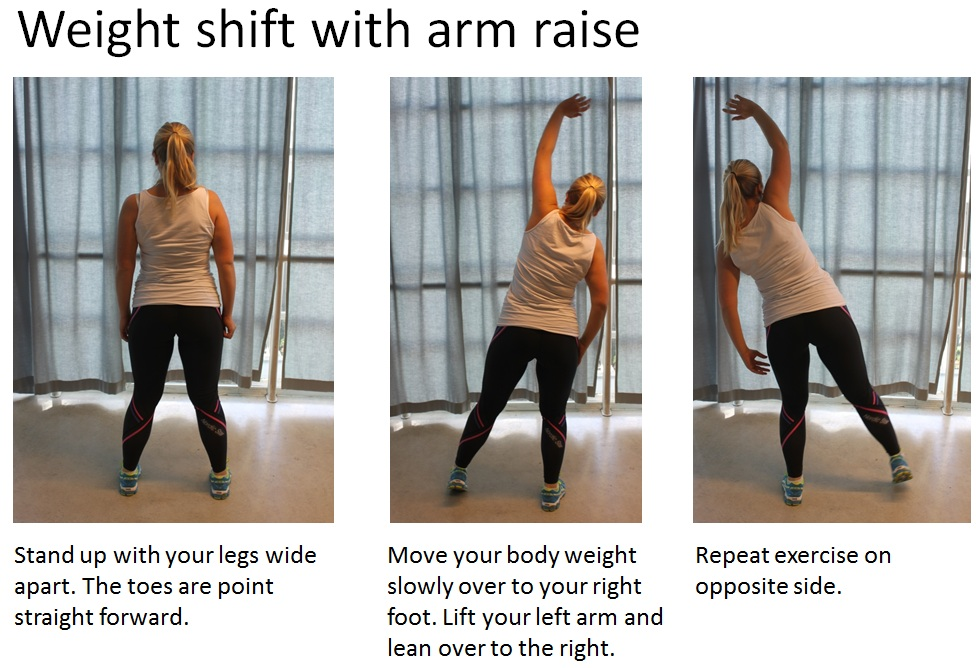
\includegraphics[scale=0.8]{WeightShift.jpg}
\label{weightshift}
\end{figure} 

\begin{figure} [H]
\centering
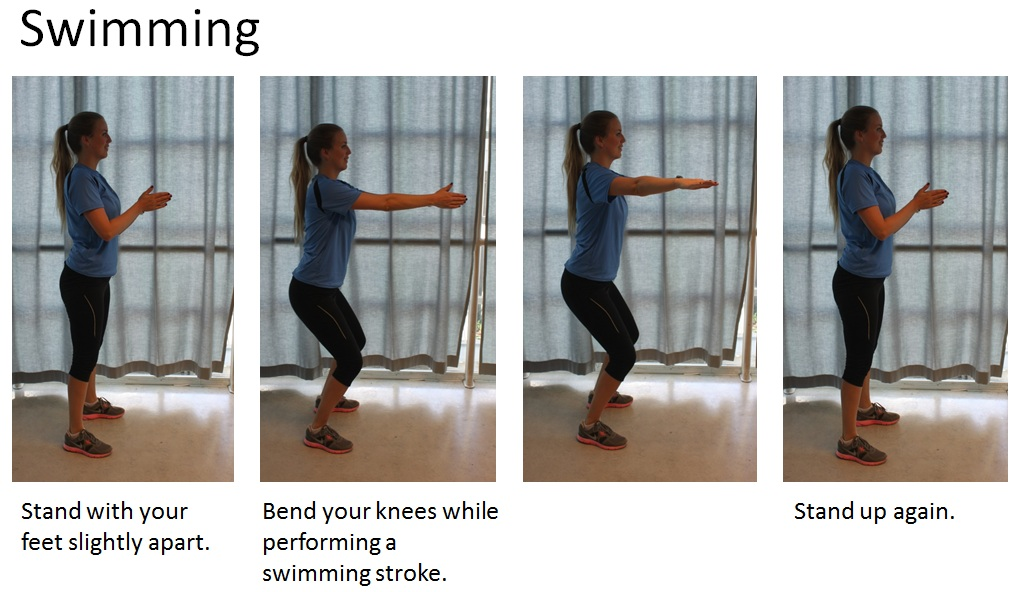
\includegraphics[scale=0.8]{Swimming.jpg}
\label{swimming}
\end{figure}

\begin{figure} [H]
\centering
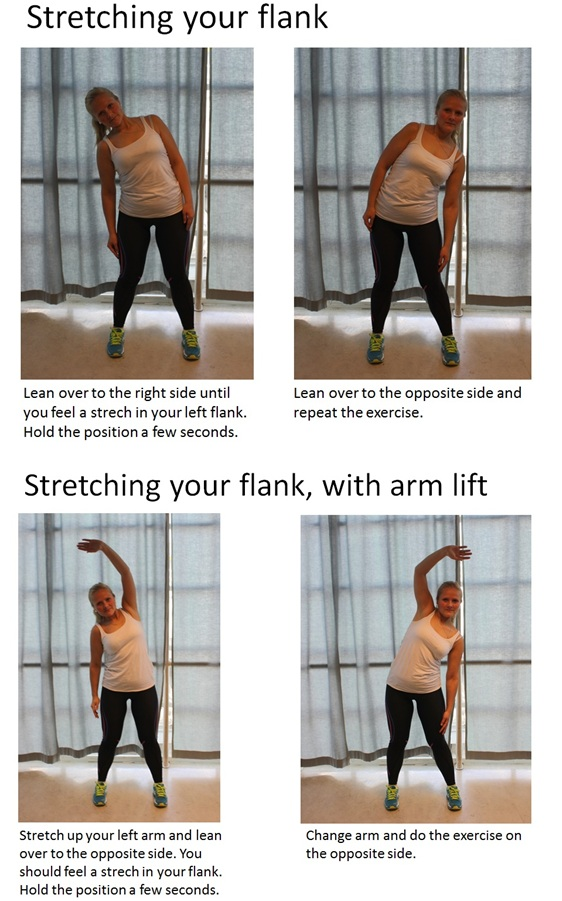
\includegraphics[scale=0.8]{StrechFlank.jpg}
\label{stretchflank}
\end{figure} 

\begin{figure} [H]
\centering
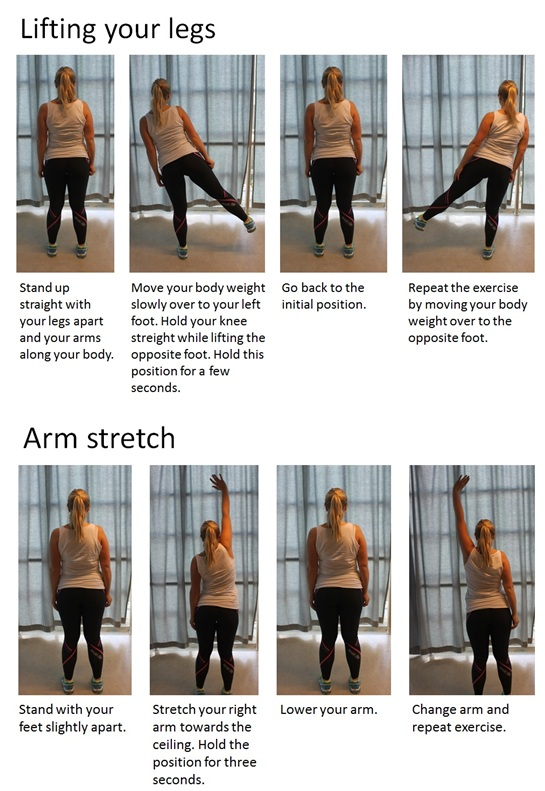
\includegraphics[scale=0.8]{LiftingYourLegs.jpg}
\label{liftlegs}
\end{figure} 


\begin{figure} [H]
\centering
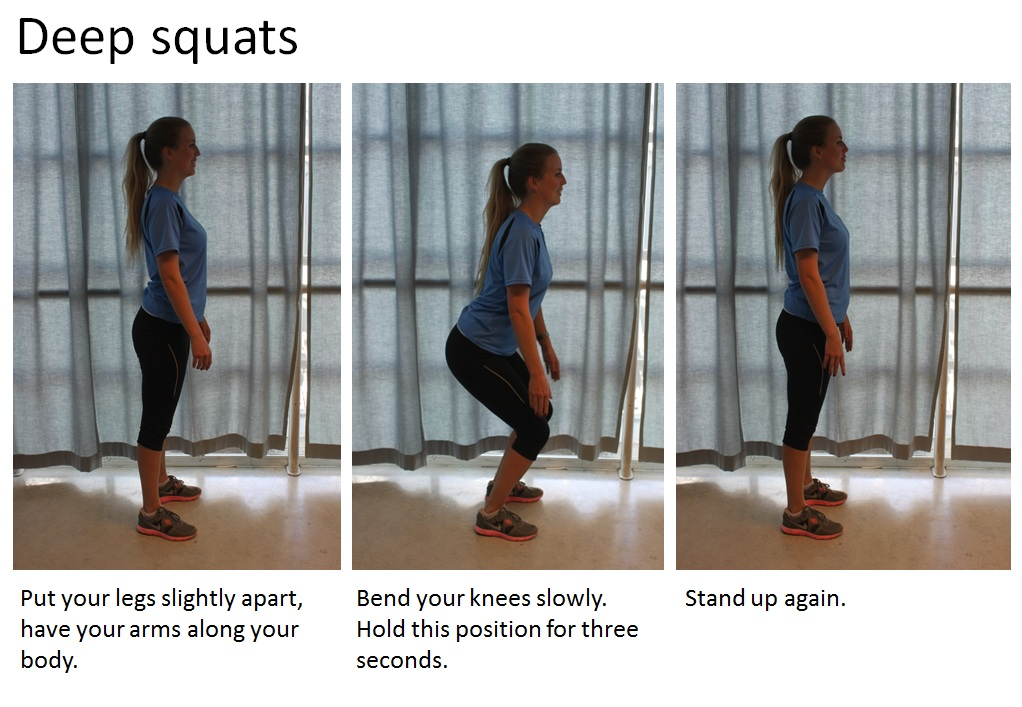
\includegraphics[scale=0.8]{Squats.jpg}
\label{squats}
\end{figure}  

\begin{figure} [H]
\centering
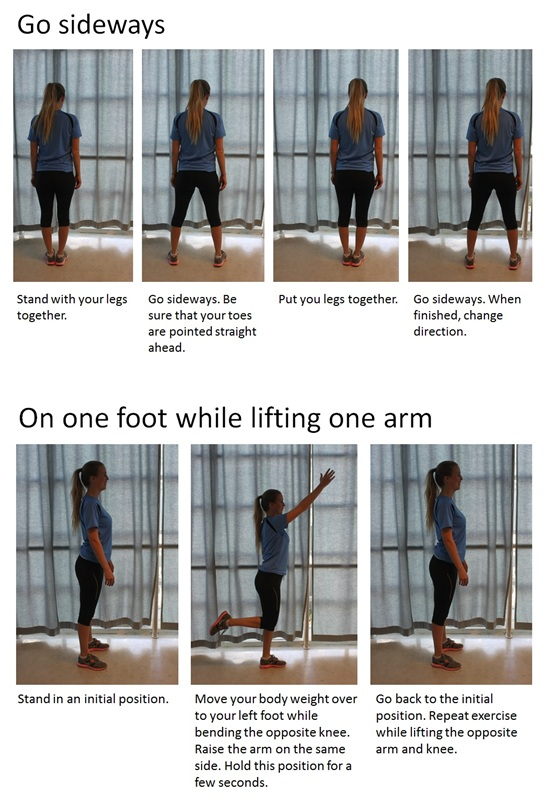
\includegraphics[scale=0.8]{GoSideways.jpg}
\label{gosideways}
\end{figure} 

\newpage
\section*{Appendix C - Review of the original Norwegian menu}
\label{app:menureview}

The figures shown in Appendix C shows a review of the original prototypes of the menu. This menu was presented for the informants in workshop 2, and is therefore in Norwegian. The menu review starts with the choice on how to play. The player chooses to play according to a preferred muscle group. A selection of single games are shown, where the player chooses "picking apples". The menu shows a start, middle, and end scene from this game. When finished, the player chooses to change number of players from single player to multi player.  

\begin{figure} [H]
\centering
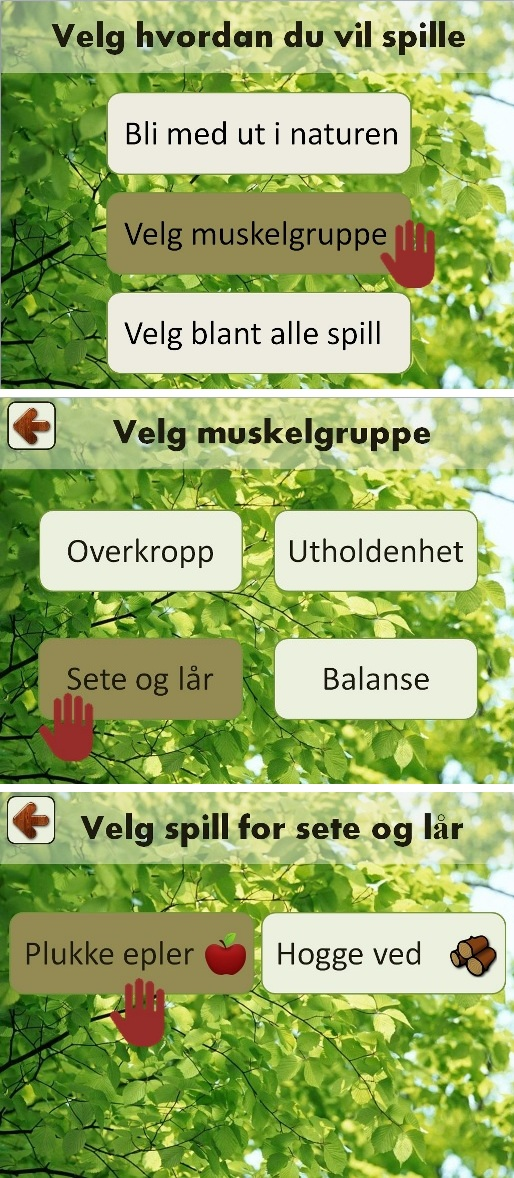
\includegraphics[scale=0.45]{menuStep1.jpg}
\label{app:menu1Norsk}
\end{figure}

\begin{figure} [H]
\centering
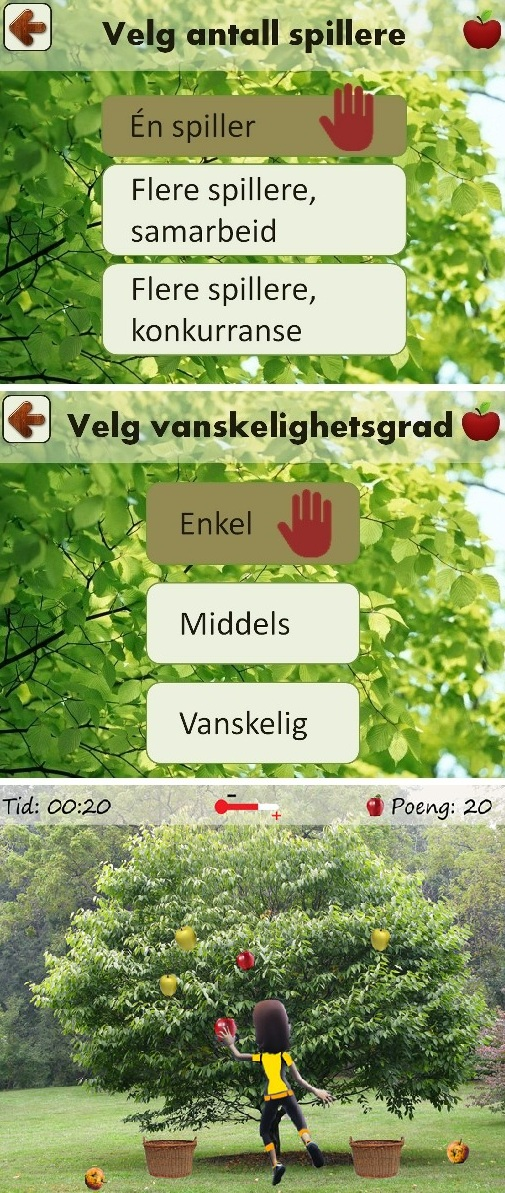
\includegraphics[scale=0.45]{menuStep2.jpg}
\label{app:menu2Norsk}
\end{figure}

\begin{figure} [H]
\centering
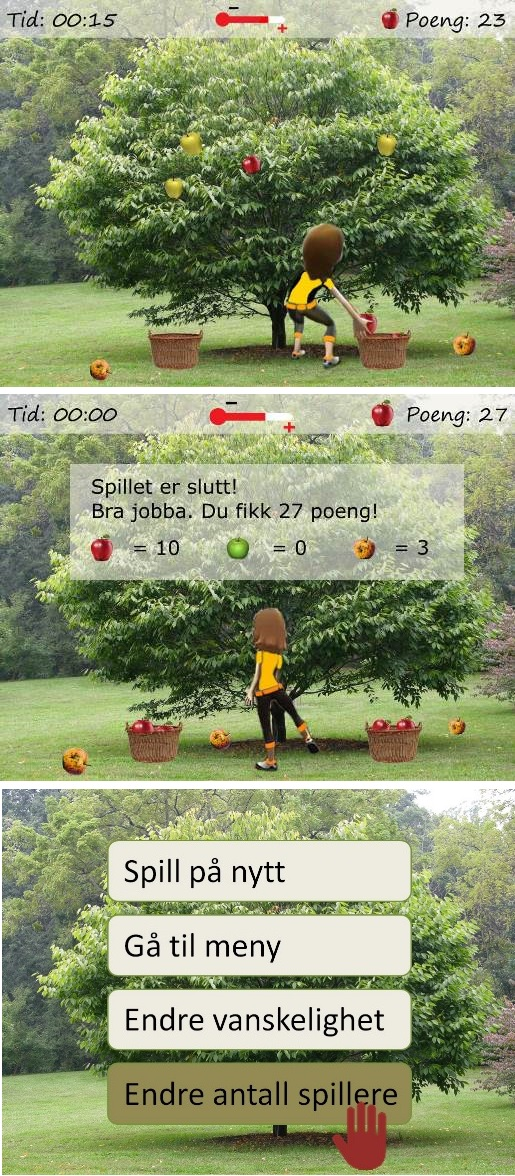
\includegraphics[scale=0.45]{menuStep3.jpg}
\label{app:menu2Norsk}
\end{figure}

\begin{figure} [H]
\centering
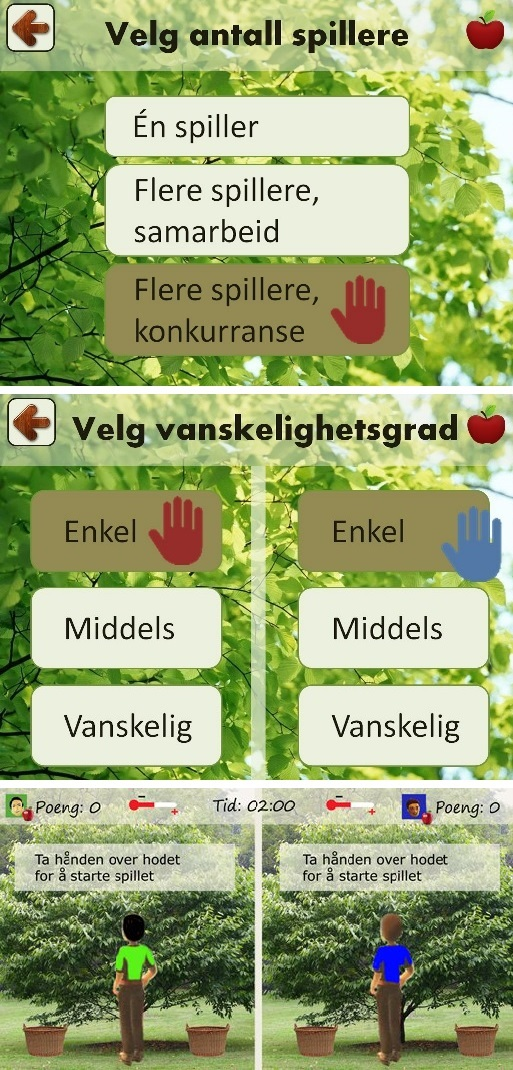
\includegraphics[scale=0.45]{menuStep4.jpg}
\label{app:menu2Norsk}
\end{figure}

\newpage
\section*{Appendix D - Various steps from the original Norwegian menu}
\label{app:menu}

\begin{figure} [H]
\centering
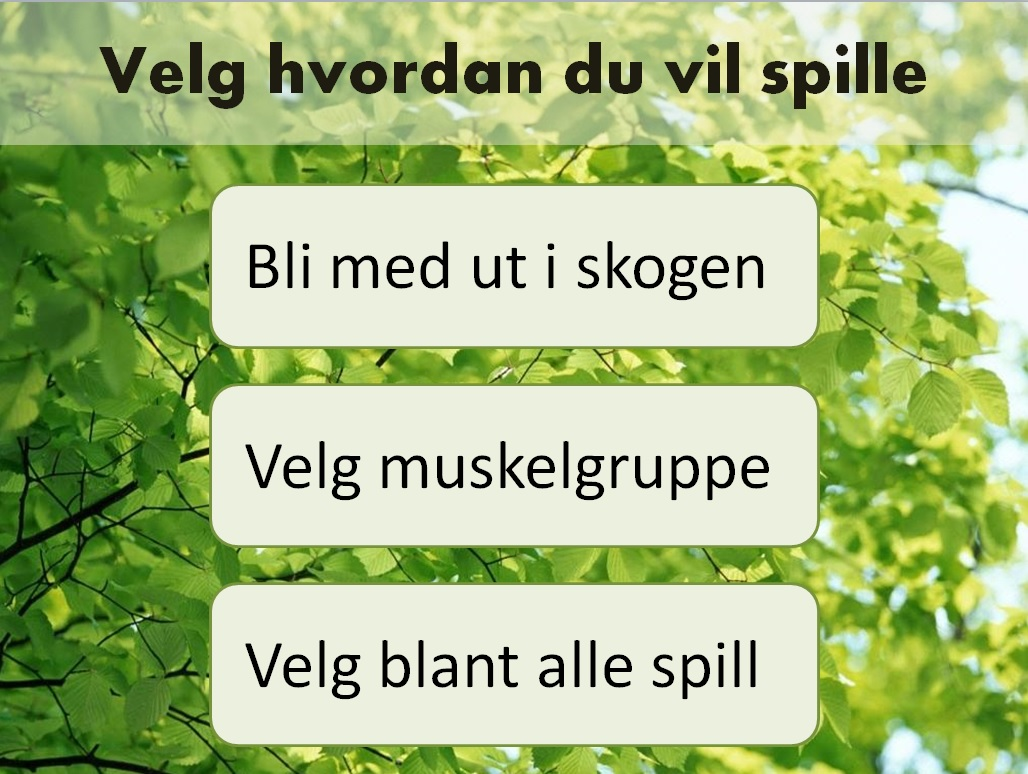
\includegraphics[scale=0.45]{menuStart.jpg}
\label{fig:menuStartNorsk}
\end{figure} 

\begin{figure} [H]
\centering
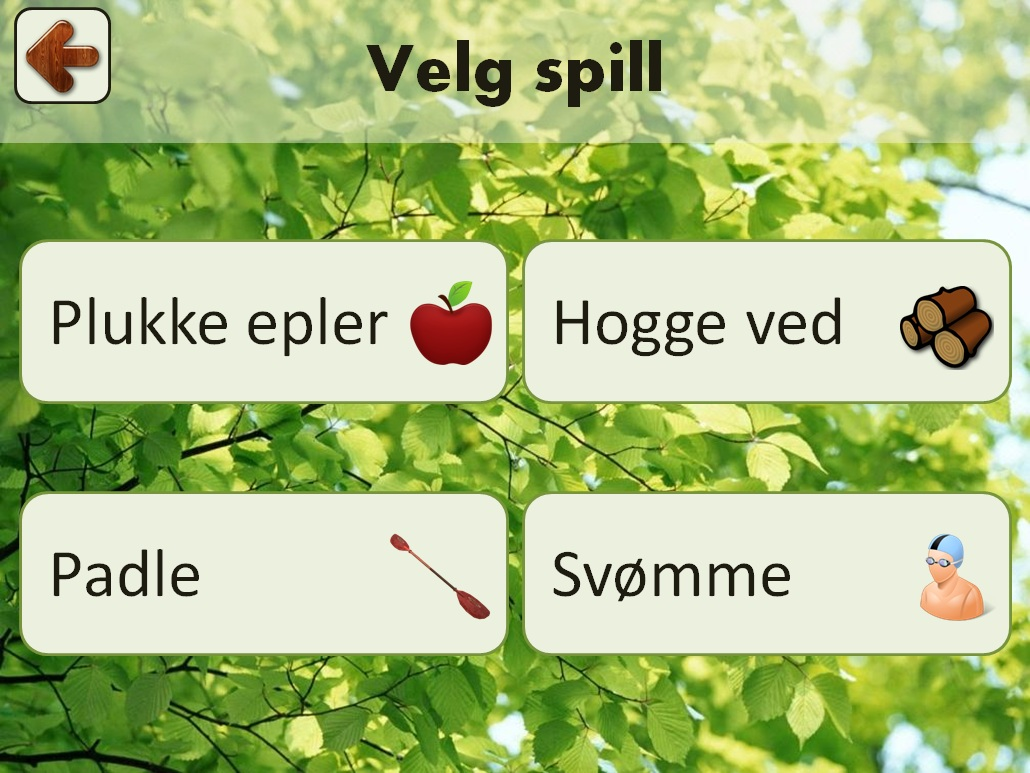
\includegraphics[scale=0.4]{VelgSpill.jpg}
\label{velgSpillNorsk}
\end{figure}

\begin{figure} [H]
\centering
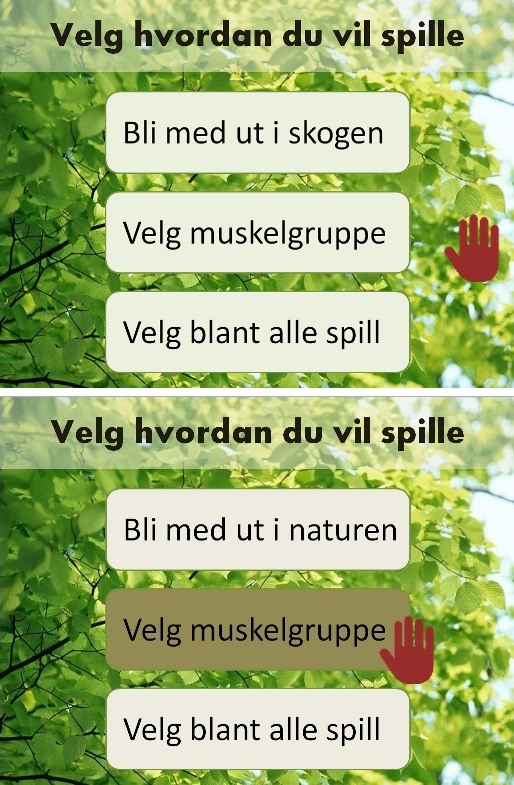
\includegraphics[scale=0.5]{menuAvatarAction.jpg}
\label{fig:avatarActionNorsk}
\end{figure} 

\begin{figure} [H]
\centering
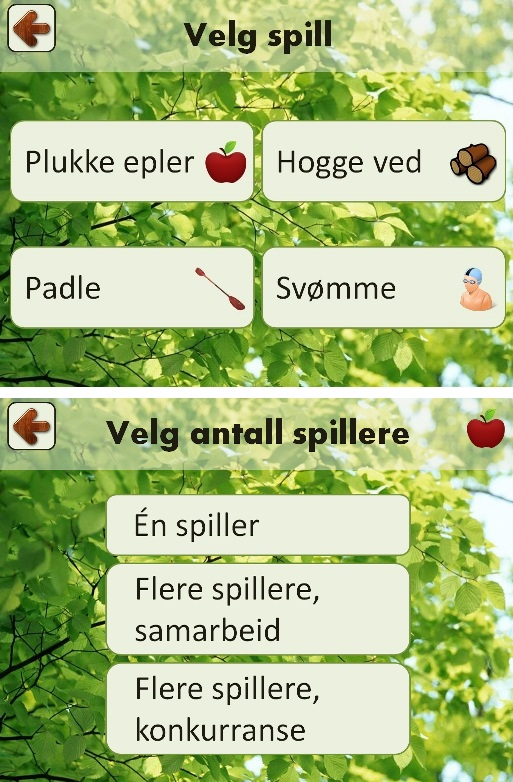
\includegraphics[scale=0.5]{IconEple.jpg}
\label{fig:iconEpleNorsk}
\end{figure} 

\begin{figure} [H]
\centering
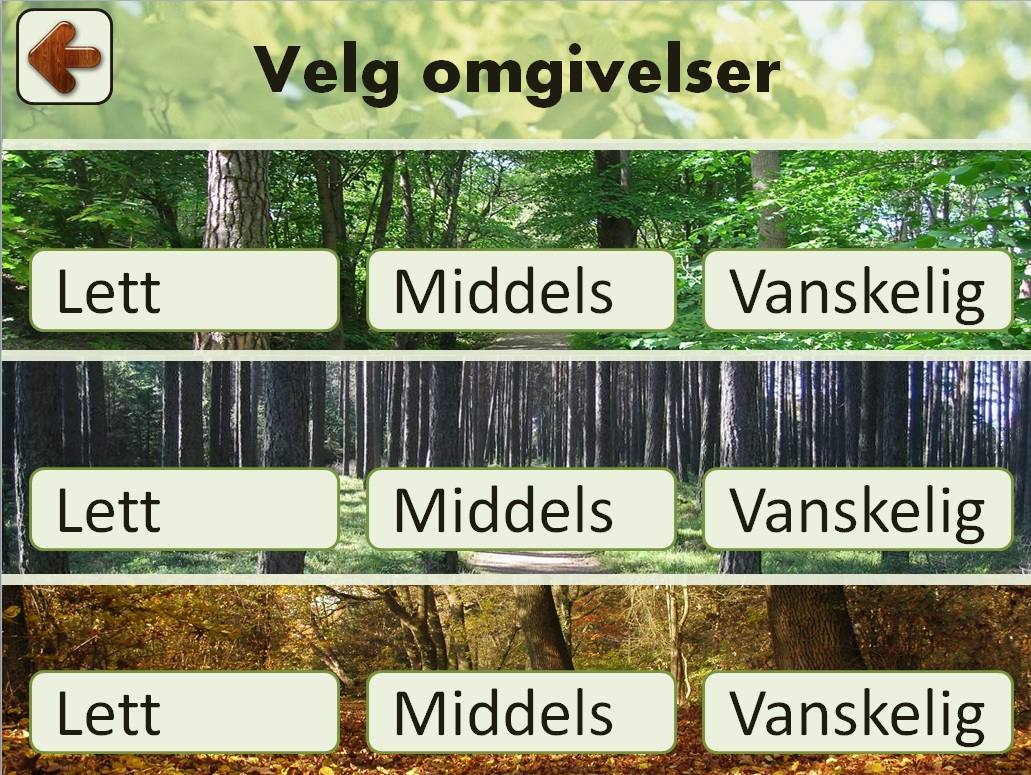
\includegraphics[scale=0.45]{VelgOmgivelser.jpg}
\label{fig:omgivelseNivaaNorsk}
\end{figure}

\begin{figure} [H]
\centering
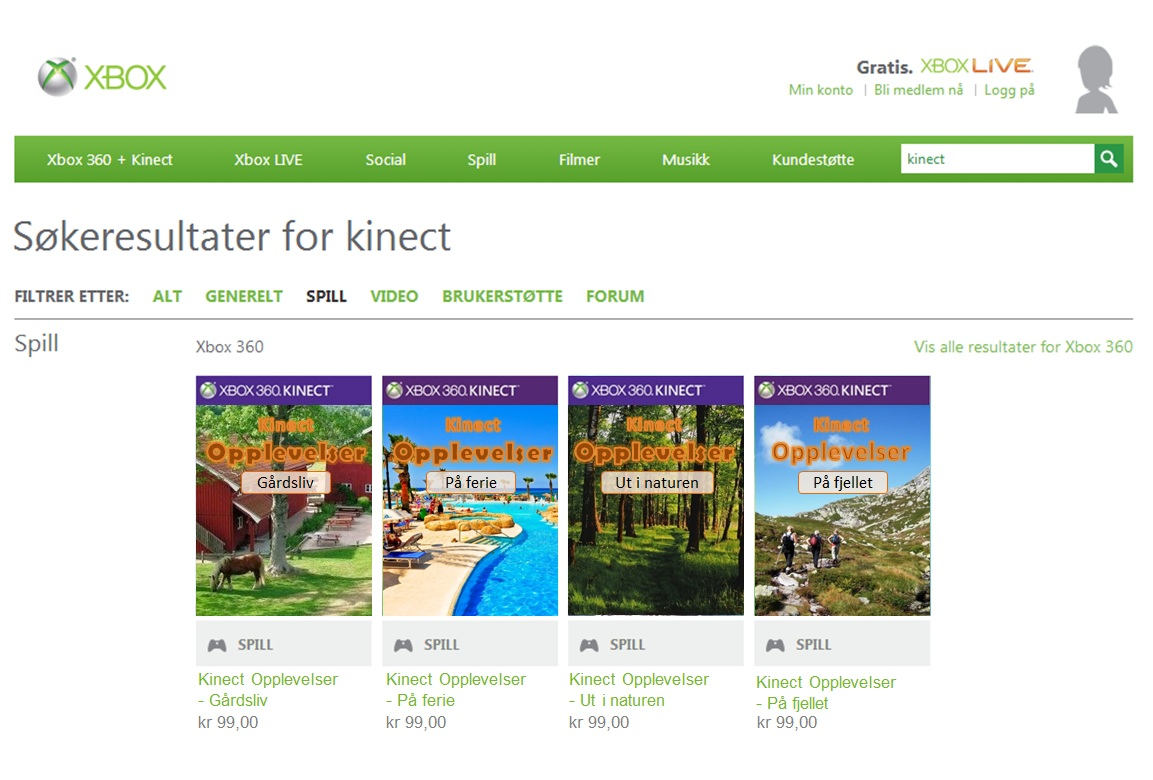
\includegraphics[scale=0.5, angle=90]{SpillXboxNYNY.jpg}
\label{fig:videogameseriesHeleNorsk}
\end{figure}